\documentclass[12pt,titlepage]{article}
\usepackage[ngerman]{babel}
\usepackage[utf8]{inputenc}

\usepackage[autostyle=true,german=quotes]{csquotes}%NC: needed for babel

\usepackage[a4paper , lmargin = {2.5cm} , rmargin = {2.5cm} , tmargin =
{2cm} , bmargin = {2cm}]{geometry}

\usepackage[hyphens]{url}
\usepackage[linktocpage=true]{hyperref}

\usepackage{tabularx}

\usepackage{amsmath}
%\numberwithin{equation}{section}

% ### Bibliographical Stuff ###
% Use \textcite{} and \parencite{} with biblatex!
\usepackage[backend=biber,
    style=numeric-comp,%alphabetic-verb,
    sortlocale=de_DE,
    natbib=true,
    url=true, 
    doi=true,
    eprint=false]{biblatex}%NC: replaced bibtex by biber
\addbibresource{literatur.bib}%Dateiname für Quellen einfügen
\usepackage{ragged2e} %für bessere URL formatierung bei printbibliography 

%Bilder einbinden und auf der gleichen seite ein
%Fußnotenzitat einzufügen
%https://en.wikibooks.org/wiki/LaTeX/Importing_Graphics
\usepackage{graphicx}
\DeclareGraphicsExtensions{.pdf,.png,.jpg} %order of preference
\graphicspath{ {../images/} } %NC: Additional path to look for images in (placed higher up to support one location for multiple documents)
%\usepackage{float} %NC: Causes problems. deactivate this and the next
%\usepackage{afterpage} %need to use with: \af­ter­page{\clearpage} https://www.ctan.org/pkg/afterpage?lang=de

\interfootnotelinepenalty=99999 %Seitenumbruch einer Fußzeile verhindern

\usepackage{moreverb} %tabulator formatierung in verbatim umgebung

%Tables:
\newcolumntype{b}{X}
\newcolumntype{s}{>{\hsize=.5\hsize}X}

\newcommand{\bildcite}[6]{
     \begin{figure}[H]
         \includegraphics[width=\textwidth]{Bilder/#1}
         \caption[#2]{#2\footnotemark}
         \label{#3}
     \end{figure}
     \footnotetext{\cite[#6][#5]{#4}}
}

\newcommand{\bild}[3]{
     \begin{figure}[H]
         \includegraphics[width=\textwidth]{Bilder/#1}
         \caption{#2}
         \label{#3}
     \end{figure}
}

\renewcommand{\labelenumi}{\arabic{enumi}.}
\renewcommand{\labelenumii}{\arabic{enumi}.\arabic {enumii}}
\renewcommand{\labelenumiii}{\arabic{enumi}.\arabic{enumii}.\arabic{enumiii}}

\newcommand{\firstpages}{
    % \input{0_Deckblatt.tex}

     \newpage
     \tableofcontents{}
     \addtocontents{toc}{~\hfill\textbf{Seite}\par}

     \newpage
     \listoffigures

     \newpage
     \listoftables
     \newpage
}


\begin{document}
\title{\huge{Wirtschaftlichkeit von energieeffizienten Netzkonzepten} \\ \large{Exposé}} 
\author{Veronika Lawrence, Carmen Scheer, Nicholas Cariss, Maximilian Junker,\\ Christian Keck, Stefan Ludowicy, Dominik Schneider} 
\maketitle
\firstpages
%\twocolumn
\section{Stand der Forschung}
Gegenstand der Projektarbeit bildet ein hinsichtlich der Energieeffizienz und Wirtschaftlichkeit zu optimierendes Carrier-Netzwerk.

Unter einem Carrier "`versteht man […] eine Gesellschaft, die mindestens drei Übertra\-gungs\-wege betreibt, die über eine Vermittlungsstelle miteinander verbunden sein müssen"' (aus: \cite{carrier}). Ein Carrier-Netzwerk stellt somit physikalische Transportwege und -verfahren zur Verfügung und bildet die Grundlage für sogenannte Value Added Services von Providern, welche auf den Carrier-Diensten aufsetzen \cite{fassnacht}. "`Bei den TK-Transportwegen unterscheidet man leitergebundene Verbindungen auf der Basis von Kupferkabeln oder Lichtwellenleitern sowie Funkverbindungen wie Satellitenverbindungen, Richtfunkstrecken und Rundfunkverbindungen"' (Aus: Ebd.).

Somit umfasst ein Carrier-Netzwerk nicht nur das physikalische Backbone-Netz, sondern auch das Zugangs- und Aggregationsnetzwerk. Im Rahmen des Projektes entfällt die Betrachtung der Optimierungspotentiale des Zugangsnetzes zugunsten einer aus\-führ\-lich\-eren Simulation von wirtschaftlichen und energieeffizienten Netzkonzepten im Backbone- und Aggregationsnetzwerk. So bildet der Broadband Network Gateway (BNG) die niedrigste Netzelementebene. Multi-Service Access Nodes (MSAN), Digital Subscriber Line Access Multiplexer (DSLAM), enhanced NodeBs (eNodeB) und weitere Netzelemente der nächsttieferen Hierarchiestufe fallen somit aus der Betrachtung.


\subsection{Energieverbrauch in Netzwerken}
Um den Energieverbrauch im Carrier-Netzwerk berechnen zu können, bedarf es an Werten der im Backbone verwendeten Netzkomponenten. Innerhalb der Simulation wird für die Berechnung des Gesamtverbrauchs auf die definierten Werte zurückgegriffen, die in einer Datenbank gespeichert sind. Ziel dieser Arbeit ist die Simulation und Berechnung des gesamtheitlichen Energieverbrauchs. Deshalb verwendet die Berechnung die von den beiden Wissenschaftler Ward Van Heddeghem und Filip Idzikowski in ihrer Veröffentlichung \cite{vanhedde} zusammengetragenen Werte. Die Quelle beinhaltet zum einen das analytische Model der Berechnung und zum anderen ein Datenblatt \cite{vanhsheet} des Energieverbrauchs der unterschiedlichen Hersteller. Das Datenblatt gliedert die Geräte nach den Unterschiedlichen Layer IP/MPLS, Ethernet, OTN, WDM - (OSI-Layer: 3-2-1-1). Zu beachten ist beim Verwenden der Werte, dass es sich um Werte unter typischen Lastbedingungen handelt, die sich nach der Kapazität der Komponente richtet und nicht nach dem aktuellen Durchsatz. Des Weiteren geben die Werte nur dein Stromverbrauch für den Betrieb an, ein Verbrauch für Kühlung o.Ä. ist nicht enthalten.
Der Gesamtverbrauch des Core-Networks ergibt sich aus der Summe alle Verbrauche der einzelnen Schichten. 

\begin{equation}
P_{core} = P_{ip} + P_{ethernet} + P_{otn} + P_{wdm}
\end{equation}


\subsection{Energie-effiziente Technologien}
Der aktuelle Stand der Forschung bietet verschiedene Konzepte und Technologien für das Einsparen von Energie in Carrier-Netzen. In dieser Arbeit sollen ausgewählte Konzepte und Technologien genutzt werden, um die Wirtschaftlichkeit von energieeffizienten Netzen zu analysieren. Betrachtet wurden im Rahmen der Literaturrecherche die folgenden Konzepte und Technologien: 

Das erste Konzept sieht eine Vereinfachung des Netzes vor, welche durch eine geographische Aufteilung des Netzes in Submodale (Global - Kontinental - National - Regional - Zugang) erfolgen kann \cite{aleksic2014}.

Das zweite Konzept befasst sich mit der dynamischen Abschaltung unterlasteter Netzkomponenten. Tageszeitabhängige Schwankungen des Traffics in Netzen ermöglichen eine individuelle und dynamische Abschaltung von Switches und Links unter der Be\-rück\-sich\-ti\-gung der QoS-Bedingungen \cite{aleksic2013}. Dabei werden Algorithmen zur Identifikation von individuell abschaltbaren Links verwendet \cite{fisher}.

Bei den Technologien beschränkt sich diese Arbeit auf optische leitungsvermittelnde Switche und das Hybrid Optical Switching (HOS). Optische leitungsvermittelnde Switche basieren auf mikro-elektromechanischen Systemen, die die geringste Menge an Energie benötigen und eine hohe Portanzahl besitzen. Das Hybrid Optical Switching verwendet eine Kombination aus optischen und elektronischen Netzknoten, die optische Leitungen, Bursts, und Pakete effizient Switches können. Durch die Kombination von langsamen und schnellen Switches, können Wellenlängenbereiche dynamisch zwischen zwei Switches geändert werden. Das temporäre Abschalten von ungenutzten Ports des schnellen Switches ermöglicht eine Energieeinsparung.  \cite{aleksic2013}

\section{Problemstellung und Motivation}
Nach einer Schätzung des ICT-Analysehauses Gartner erzeugte die Informations- und Kommunikationstechnologie im Jahr 2007 rund 2\% des globalen Ausstoßes an CO2, was dem Ausstoß der Flugzeugbranche entspricht \cite{gartner}. Seit dem ist der Anteil der Bevölkerung weltweit, der das Internet verwendet, von 20,6\% (2007) auf 43,4\% (2015) gestiegen \cite{itu}. Dieses Wachstum wird sich in der nächsten Zukunft nicht verlangsamen. Es ist also unabdingbar, den CO2-Ausstoß, der durch ICT im Allgemeinen verursacht wird, drastisch zu verringern.

\begin{figure}[!ht]
    \centering
    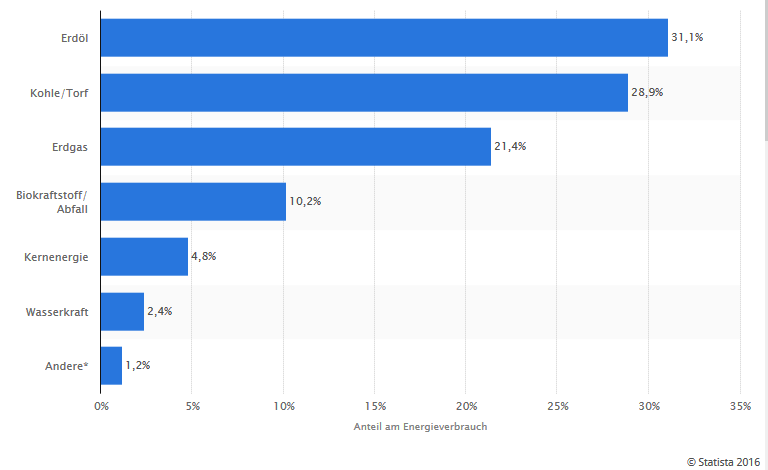
\includegraphics[width=0.8\textwidth]{statista}
    \caption{Verteilung der weltweiten Energieerzeugung nach Energieträger im Jahr 2013 (Quelle: statista)}
    \label{fig:statista}
\end{figure}

Da aller Bemühungen zum Trotz die fossilen Energieträger Erdöl, Kohle und Erdgas weiterhin ca. 81\% der weltweiten Energieerzeugung ausmachen \cite{statista}, ist die Reduktion des Energieverbrauchs von ICT-Infrastruktur ein wichtiger Ansatz, um den CO2-Ausstoß zu verringern. Natürlich sind neben dem Bemühen, ICT grüner zu gestalten, wirtschaftliche Bedenken ein weiterer wichtiger Treiber für das Streben nach mehr Energieeffizienz. Langfristig steigende Energiekosten (\cite{iea2015}, S. 40f) sind ein großes Risiko für ICT-Provider weltweit, die insgesamt mit steigenden Kosten zu kämpfen haben.
 
Die vorliegende Arbeit beschränkt sich auf die ökonomischen Zwänge, die sich aus ineffizienten Netzen ergeben. Es soll eine Software entwickelt werden, die es ermöglicht, zwei hypothetische Netze miteinander zu vergleichen, zum einen ein konventionelles Netz, wie es heutzutage Stand der Technik ist, zum anderen ein energieeffizientes Netz, das die vorhandenen Technologien und Konzepte zur Effizienzsteigerung sinnvoll einsetzt. Anhand des berechneten Energieverbrauchs der beiden Netze wird das Energiesparpotenzial sowie die möglichen Kosteneinsparungen durch den Betrieb des energieeffizienten Netzes ausgegeben.


\section{Methodisches Vorgehen}
Zur Durchführung einer Kalkulation des Energiesparpotentials und möglicher Kostenersparnisse durch Verwendung von energieeffizienten Netztechnologien und -konzepten wurde folgendes methodisches Vorgehen entwickelt. 
 
Zunächst sollen im Rahmen der Literaturrecherche Methoden für die Reduzierung des Energieverbrauchs und die Erhöhung der Energieeffizienz in Kommunikationsnetzen ermittelt werden. In einem weiteren Schritt gilt es alle gefundenen Technologien zu konsolidieren, das Netz zu spezifizieren und verschiedene Szenarien, die anschließend verglichen werden sollen, zu definieren. 
 
Bei der Spezifikation des Netzes liegt ein Hauptaugenmerk auf der Eingrenzung des für diese Arbeit relevanten Scopes. Im Rahmen dieser Arbeit soll dabei ein komplettes Carriernetzwerk modelliert, bezüglich Einsparpotentialen jedoch nur das Core-Netz betrachtet werden.
 
Zur Vorbereitung der Entwicklung der Simulationssoftware müssen darauf folgend Szenarien (zum einen ein Business-As-Usual- und ein energieeffizientes Netz) modelliert werden. Wichtig ist dabei zu klären, aus wie vielen und welchen Netzkomponenten das jeweilige Netz besteht, welche Nutzungsprofile für die Simulation verwendet werden und welche Konfigurationsmöglichkeiten der Anwender der Simulationssoftware haben soll. 
 
Anschließend sollen der Gesamtenergieverbrauch des jeweiligen Netzes sowie die potenziellen Kostenersparnisse durch die Erhöhung der Energieeffizienz abgeschätzt werden. Dazu gilt es insbesondere einen "`Algorithmus"' zu entwickeln, der basierend auf variablen Eingabeparametern den Energieverbrauch eines Netzes berechnet. 
 
Auf Grundlage dieser Entscheidungen und Planung soll dann der Prozess der Softwareentwicklung beginnen, der nach dem Wasserfallmodell ablaufen wird. Die Programmaufteilung und geforderte Funktionen sind bereits vor der Implementierung hinreichend bekannt, so dass die Anwendung eines agilen Entwicklungsmodells hier keine entscheidenden Vorteile bietet.
 
Die Softwarelösung wird als objektorientierte Java Desktop Anwendung mit einer Einteilung der Klassen in die drei Bereiche Model, View und Controller implementiert.
 
Der Bereich Model beinhaltet das Einlesen so wie auch die Manipulation von Netzlast-Werten, Hardwarekonfigurationen und sonstigen für die Berechnung notwendigen Daten aus einer im Rahmen dieses Projektes entwickelten MySQL-Datenbank. Die in der Simulation errechneten Ergebnismengen werden in diesem Bereich gespeichert und auch die finale Datenbewertung ("`Geschäftslogik"') wird hier implementiert.
 
Der Bereich View beinhaltet die Anwendungsformulare zur Bearbeitung der Netz\-hard\-ware- und Verbindungs-Kon\-figura\-tion, zur Auswahl von Konfigurationsparametern für die Simulation und zum Anzeigen der berechneten Ergebnisse. Das Ergebnis der Simulation wird in Form von Tabellen (z.B. Iterationsnummer | Netzlast | elektr. Stromverbrauch | \% von Maximalverbrauch) und mehrerer Diagramme (jfreechart) im Anwendungsfenster angezeigt. Die Diagrammerstellungs- und Anzeigefunktionen werden auch in diesem Bereich abgelegt.
 
Der Bereich Controller beinhaltet die Anwendungslogik, die Implementierung des Portabschaltungsalgorithmus "`Exhaustive Greedy Algorithm"' (bei Erfüllung der Netzlast-Anforderungen, Einhaltung eines vom Anwender der Simulationssoftware festgelegten maximalen Hop-Counts und die verschachtelten Schleifen zum durchprobieren der Lösungs\-möglich\-keiten (Netzlast-Routing und Energiespar-/Ab-schaltung von Netzwerkstrecken) mit dem Ziel der Findung des besten Ergebnisses (früher Abbruch einer Schleifeniteration, wenn die Vorgaben nicht mehr eingehalten werden oder der Gesamtstromverbrauch einer Lösung einer früheren Iteration überschritten wurde). Um ein Ergebnis im Zeitlichen Verlauf abhängig von den konfigurierten Netzlast-Daten zu erzielen wird iterativ je zeitlichem Abschnitt die Lösungsberechnung durchgeführt und in Ergebnistabellen eingetragen.
 
Allgemein findet nur eine sehr rudimentäre Validation der Benutzereingaben statt. Beispielsweise liegt es in Verantwortung des Anwenders, keine für das konfigurierte Netz zu große Netzspitzenlast zu konfigurieren. (Out of Scope) In einer späteren Weiterentwicklung könnte eine komplexe Plausibilitätsprüfung implementiert werden.
 
Diese Aufteilung der einzelnen Implementierungsaspekte erlaubt eine Verteilung der Entwicklungsarbeit auf die Projektmitglieder, so dass diese voneinander weitgehend unabhängig an der Implementierung arbeiten und die jeweiligen Entwicklungsfortschritte über ein git Repository auf https://github.com/EnergyNetSim/Simulator verteilen können. Der jeweilige Entwicklungsfortschritt ist spätestens alle 3 Tage und bei Fertigstellung einzelner Teilfunktionen auf das git Repository zu commiten und pushen.

\section{Projektmanagement und Zeitplan}
In Anbetracht der genau festgelegten Terminstruktur des Moduls wurde entschieden, das Projektmanagement mit klassischen Methoden (in Anlehnung an IPMA ICB 3.0 \citep{icb}) durchzuführen. Im folgenden seien die Arbeitspakete sowie die Ablauf- und Terminplanung des Projekts exemplarisch gemäß ihrem aktuellen Stand genannt. 
 
\subsection{Arbeitspakete}

\begin{enumerate}
\item Vorbereitung
\begin{itemize}
\item Analyse der Aufgabenstellung
\item Projektplanung / -vorbereitung
\item Tools und Kommunikation festlegen
\item Entwicklungsumgebung aufsetzen
\end{itemize}

\item Literaturrecherche
\begin{itemize}
\item Recherche zu Methoden für die Reduzierung des Energieverbrauchs und die Erhöhung der Energieeffizienz in Kommunikationsnetzen
\item Projektplanung / -vorbereitung
\item Tools und Kommunikation festlegen
\end{itemize}

\item Modellierung des Netzwerks
\begin{itemize}
\item Spezifikation eines Netzes
\item Definition der Szenarien (BAU und energieeffizient)
\end{itemize}

\item Softwareentwicklung
\begin{itemize}
\item Anforderungsanalyse
\item Spezifikation
\item Systemdesign
\item Programmierung
\item Test
\end{itemize}

\item Projektdokumentation
\begin{itemize}
\item Gliederung
\item Zusammenfassen der in den anderen Phasen dokumentierten Ergebnisse
\item Abschätzung des Gesamtenergieverbrauchs des Netzes für die zwei Szenarien
\item Abschätzung der potenziellen Kostenersparnisse durch die Erhöhung der Energieeffizienz
\item Diskussion der Ergebnisse
\end{itemize}

\item Präsentation
\begin{itemize}
\item Folien erstellen
\item Probeläufe
\item Präsentation halten

\end{itemize}

\item Projektmanagement
\begin{itemize}
\item Ständige Dokumentation der Aktivitäten
\item Kooperation, Kommunikation, Koordinierung im Team
\item Fortschrittskontrolle
\item Qualitätskontrolle, Risikoüberwachung, Quality Gates
\end{itemize}

\end{enumerate}
 
\subsection{Ablauf- und Terminplanung}
Die Ablaufplanung ist in Abbildung \ref{fig:gantt} beschrieben und im Ganttchart mit Terminen hinterlegt.
\begin{figure}[!h]
    \centering
    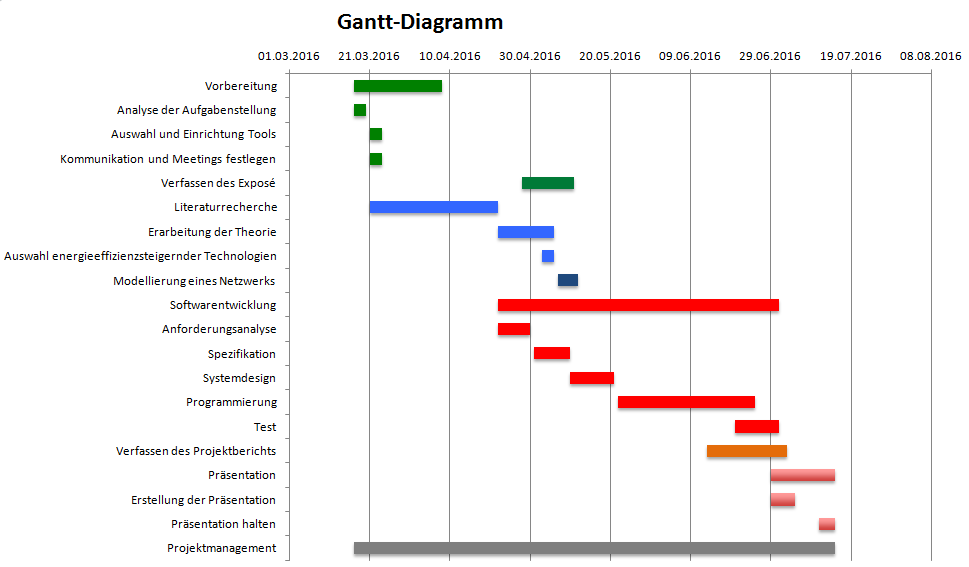
\includegraphics[width=0.8\textwidth]{gantt}
    \caption{Ablauf- und Terminplan als Gantt-Chart}
    \label{fig:gantt}
\end{figure}

 \subsection{Meilensteine}
Die Meilensteine des Projekts können Tabelle \ref{tab:milestones} entnommen werden.
 

 
 \begin{table}[h]
    \centering
    %\begin{tabularx}{\textwidth}{| X | X | X |}
    \begin{tabular}{|c || c c|} 
        \hline
        Name     & Beschreibung     & Datum     \\ 
        \hline \hline
        M1         & Teletutoring 1        & KW 14         \\ 
        M2 & Teletutoring 2	& KW 16\\ 
M3 & Präsenzphase	& KW 17\\ 
M4 & Teletutoring 3	& KW18\\ 
M5 &Teletutoring 4	&KW20\\ 
M6 &Teletutoring 5	&KW22\\ 
M7 &Präsenzphase	&KW23\\
M8 &Ende AZ-Woche	&KW25\\
M9 &Teletutoring 6	&KW27\\ 
M10 &Abgabe Projektbericht	&TBA (KW27)\\ 
M11 &Abgabe Präsentation/Code	&TBA (KW28)\\ 
M11 &Präsentation	& KW28\\ \hline
    \end{tabular}
    
    \caption{Meilensteine}
    
    \label{tab:milestones}
\end{table}


\newpage
\printbibliography 

\end{document}